\begin{frame}[allowframebreaks]{\underline{Introduction} -}
    \section{Introduction}
    
\begin{itemize}
\item In a recent decade, computational techniques have become more reliable.
\item Aerodynamics Shape Optimization is computational expensive job.
\item The goal of ASO is to improve the aerodynamic characteristics, resulting in increased fuel efficiency.
\item ASO approach involves using optimization
algorithms in combination with the CFD solver and the parameterization technique to reduce the problem’s dimension.
\item With sophisticated algorithm and computational power, it is now possible to aim for multimodal optimization. 	
\item The aerodynamic design optimization community makes a similar attempt to initiate the AIAA Aerodynamic Design Optimization Discussion Group
(ADODG).
\item The ADODG has developed a series of benchmark problems ranging from 2-D airfoil optimization on the Euler equations to the 3-D wing shape optimization based on the RANS equations.
\end{itemize}

Following are the various cases that are described by ADODG.
\begin{table}
    \centering
    \begin{tabular}{m{0.1\textwidth}>{\centering}m{0.04\textwidth}>{\centering}m{0.62\textwidth}>{\centering\arraybackslash}m{0.11\textwidth}}\hline
    \textbf{Figure} & \textbf{Case} & \textbf{Description} & \textbf{References} \\\hline
    \center{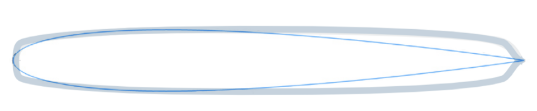
\includegraphics[width=20mm, height=8mm]{figures/case_1.png} }    & 1 & Sectional optimization of a modified NACA 0012 airfoil at zero angles of attack in inviscid, transonic flow. & \cite{case_60,case_1b,case_49}\\\hline
    \center{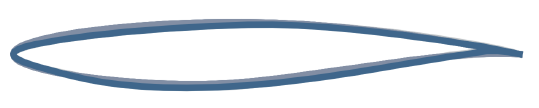
\includegraphics[width=20mm, height=8mm]{figures/case_2.png} }     & 2 & Sectional optimization of an
RAE 2822 airfoil in viscous, transonic flow. & \cite{case_60,case_1b,case_44,case_46} \\\hline
    \center{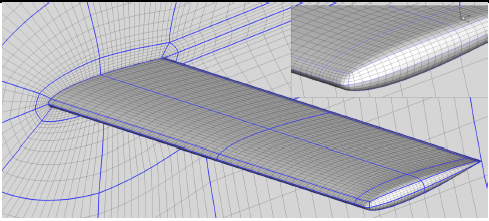
\includegraphics[width=20mm, height=10mm]{figures/case_3.png} }     & 3 & Twist optimization of a rectangular wing in subsonic, inviscid flow. & \cite{case_44,case_46,case_49}\\\hline
    \center{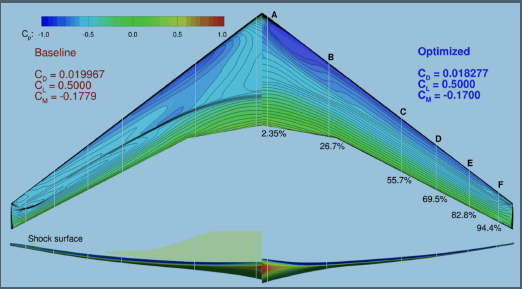
\includegraphics[width=20mm, height=10mm]{figures/case_4.png} }     & 4 & Sectional and twists optimization of the Common Research Model (CRM) wing in transonic,
viscous flow. & \cite{case_44,case_46,case_49,case_60}\\\hline
    \center{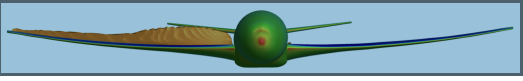
\includegraphics[width=20mm, height=10mm]{figures/case_5.png} }     & 5 & Lift-constrained drag minimization of the CRM wing-body-tail configuration at flight Reynolds number. & \cite{case_60,case_62}\\\hline
    \center{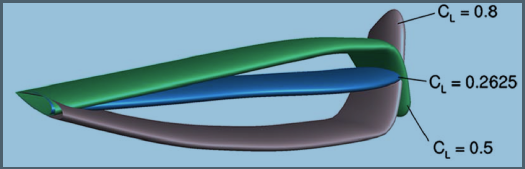
\includegraphics[width=20mm, height=10mm]{figures/case_6.png} }     & 6 &\textbf{ Multimodal subsonic inviscid lift-constrained drag minimization.} & \cite{case_63,case_64}\\\hline
    \end{tabular}
    \caption{ADODG benchmark cases}
    \label{adodg cases}
\end{table}
\end{frame}